\chapter{Anden Iteration}
I dette afsnit beskrives 2. iteration af design- og implementeringsfasen. Den indebærer design og vikling af transformator samt valg af resterende komponenter i kredsløbet. Yderligere realiseres og testes hele kredsløbet for første gang i 2. iteration.

\section{Transformator}
Transformeren fungerer anderledes ved en flyback end ved de fleste andre SMPS, hvor der løber en strøm i de primære og sekundære viklinger på samme tid. Det er ikke tilfældet ved en flyback konstruktion. Her løber strømmen kun i en vikling af gangen. Når MOSFET’en er on, vil strømmen igennem den primære vikling rampe op i forhold til indgangsspændingen og induktansen i viklingen. Pga. dioden og polariteten af den sekundære vikling, vil der på dette tidspunkt, ikke løbe en strøm i den vikling. Når transistoren går off falder strømmen i den primære vikling til 0, som får spændingerne over viklingerne til at skifte polaritet. Med en modsat polaritet på sekundærsiden, kan der nu løbe en strøm gennem dioden. 


\noindent Normalt kan energien fra den primære vikling transformeres direkte over i den sekundære vikling, da der løber en strøm på samme tid. Da det ikke er tilfældet ved flyback, kræver konstruktionen, at transformeren kan opbevare energien fra den primære vikling, indtil det kan transformeres over i den sekundære vikling. Det gør at der i transformeren er behov for et air gap, for at transformeren ikke skal gå i mætning. 


\noindent Det er fluxændringen i kernen, der sørger for, at der induceres spænding over i den sekundære vikling. Det vil sige, at der er behov for at fluxen i kernen ændrer sig forholdsvis lineært, hvilket sker når der ligger en konstant spænding over viklingen. Kernen siges at have nået mætning, når en ændring i H-feltet ikke længere ændrer lineært på fluxen. 


\noindent For at sikre ens transformatoren ikke går i mætning bruges hysteresekurven (ses på figur~\ref{fig: Hysteresekurve}) som plotter H-feltet på x aksen og B-feltet op ad y aksen. Her skal det undgås at transformatoren kommer til at blive vandret i top eller bund, da det er her, at transformatoren går i mætning. Yderligere fås et overblik over selve transformatortabet ud fra samme kurve. Det areal, som kurven indeholder, er nemlig tabet i transformatoren per switchperiode. Det betyder ligeledes, at kernetabet bliver større jo højere switch frekvens der benyttes. 

\begin{figure}[H]
	\center
	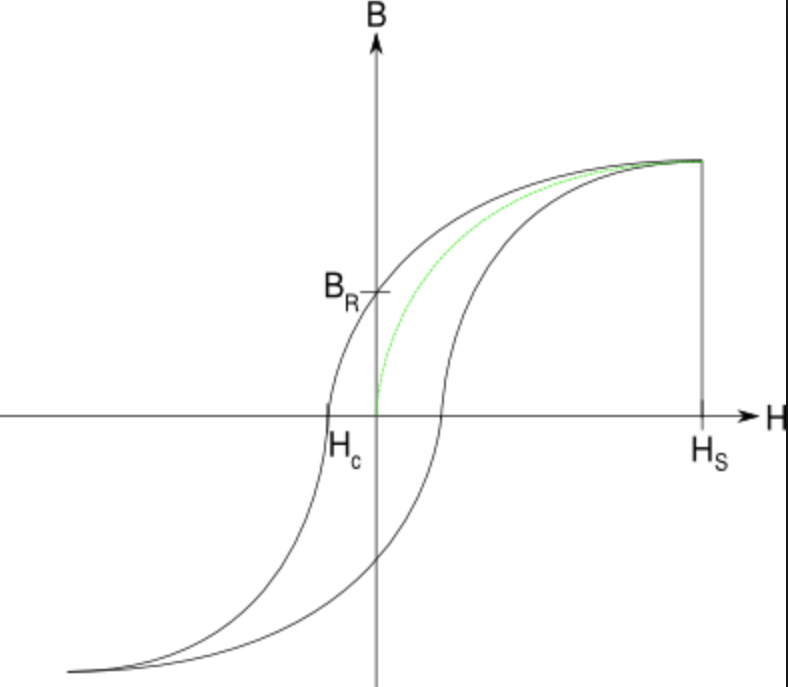
\includegraphics[max width=0.7\linewidth]{/tex/2iteration/billeder/Hysteresekurve.png}
	\caption{Hysteresekurve}
	\label{fig: Hysteresekurve}
\end{figure}
\textbf{Tænker teorien her er lidt tynd, eller er det nok??}

\subsection{Design}
Først og fremmest findes ripplestrømmen, som skal løbe i transformatoren. Her er der taget udgangspunkt i, at designe den efter $60\percent$ af udgangsstrømmen. Dette er et tradeoff mellem størrelsen på ripplen og hvor høj en induktans vi får i viklingerne. Større induktans kræver flere vindinger og giver dermed mere tab.
\begin{equation} \label{I_ripple_CCM}
I_{ripple} = 0.6 \cdot \frac{V_{out} \cdot I_{out}}{V_{inmaks} \cdot   D_{min}} = 2.13A
\end{equation}
Den nødvendige induktans det kræver for at transformatoren kan rampe op til den nødvendige strøm inden for dutycyclen, udregnes på følgende måde:
\begin{equation} \label{L_CCM}
L = \frac{V_{inmin} \cdot D_{min}}{I_{ripple} \cdot f_s} = 69.43\micro H
\end{equation}
Som beskrevet tidligere skal kernen kunne opbevare den energi som kommer fra primær viklingen, når transistoren er on, for at undgå mætning. Mængden af energi i primærviklingen udregnes ved:
\begin{equation} \label{Primary_energy}
w = \frac{1} {2} \cdot L \cdot {I_{pk}}^2 = 1.083\milli J
\end{equation}
For at beregne den tilladelige mængde energi i transformatoren, skal kernen og kernematerialet kendes. Valget er her faldet på en RM8 kerne og materialet 3f3. RM8 kernens mål gør, at den lige akkurat kan være på printet højdemæssigt. Derudover har Terma tidligere brugt RM8 kerner med 3f3 og har nogle mere præcise mål på AL og air gaps, end der er på datasheets’ne. (Kræver det flere argumenter?)


\noindent Den effektive volumen Ve aflæses for RM8. På databladet for 3f3 aflæses et maks peak af B-feltet til omkring $250\milli T$. Hvis der designes efter, at transformatoren vil operere med et højere B-felt, vil man altså risikere at kernen går i mætning. Yderligere findes permeabiliteten for 3f3 materialet uden luftgap. Med disse oplysninger vil transformatoren kunne opbevare følgende energi:
\begin{equation} \label{Energy_no_gap}
w_{kerne} = \frac{1} {2} \cdot \frac{1}{\micro_e} \cdot B^2 \cdot V_e = 53\pico J
\end{equation}
Det er tydeligt at den nødvendige energi på ingen måde kan opbevares i kernen. Da ferrit kan opbevare så lidt energi som det er tilfældet, kan det estimeres at al energien vil blive opbevaret i det luftgap, der designes. Derfor kan permeabiliteten ses som $\micro_0$ i den nye beregning. Den effektive volumen deles op i luftgap og $Al$, så luftgapet kan isoleres. Med dette kan luftgapet beregnes: 
\begin{equation} \label{Airgap}
l_g = \frac{L \cdot {I_{pk}}^2 \cdot \micro_0}{B^2 \cdot A_0} = 690.98\micro m
\end{equation}
Med den ripplestrøm der i første omgang er benyttet, skal der bruges et air gap på ca. $691\micro m$. Den nærmeste air gaps værdi for 3f3 ligger på $488\micro m$ hvilket giver en Al på $160\nano H$. (Dette er ikke databladets værdi, men en værdi der er blevet givet fra Terma, som har testet databladets værdier til ikke at være korrekte.) Det vil ikke fungere, derfor udregnes en induktans, der passer til det air gap i stedet: 
\begin{equation} \label{L1}
L_1 = \frac{l_g \cdot B^2 \cdot A_0}{{I_{pk}}^2 \cdot \micro_0} = 49.035\micro H
\end{equation}
Med kendt Al og induktans kan vindingstallet beregnes. Da der i 2. iteration bruges en 1:1 transformator er dette både for primær og sekundær vikling:
\begin{equation} \label{N}
N = \sqrt{\frac{L_1}{A_L}} = 17.5 \approx 18
\end{equation}
Det passer fint med 18 viklinger på hver side, hvor induktansen igen bliver lidt anderledes når vindingstallet rundes op. 
\begin{equation} \label{L1}
L_2 = N^2 \cdot A_L = 57.76 \micro H
\end{equation}
Med fastlagt induktans kan ny ripple- og peak strøm beregnes.
\begin{equation} \label{I_ripple_CCM}
I_{ripple} = \frac{V_{inmin} \cdot D_{max}}{L_2*f_s} = 2.24A
\end{equation}
\begin{equation} \label{I_pk_CCM}
I_{pk} = \frac{V_{out} \cdot I_{out}}{V_{inmin} \cdot D_{maks}} + \frac{I_{ripple}}{2} = 5.64A
\end{equation}

\subsection{Simulering}
